\section*{Результаты измерений}

\subsection*{Измерение коэффициента усиления активной среды}
	
		\begin{table}[H]
			\caption{Напряжение на фотодетекторах в милливольтах}
			\label{tab:my-table}
			\begin{center}
				\begin{tabular}{|c|c|c|c|}
					\hline
					Измерение & U\_вх & U\_вых & Отношение\\ \hline
					Без усиления & 220   & 2.1 &  104.76	\\ \hline
					С усилением  & 200   & 2.0 &  100.00	\\ \hline
				\end{tabular}
			\end{center}
		\end{table}

\begin{center}
	Полученное усиление:\\
	G = 1.0476
\end{center}

\subsection*{Поляризация лазерного луча}

\begin{figure}[H]
	\centering
	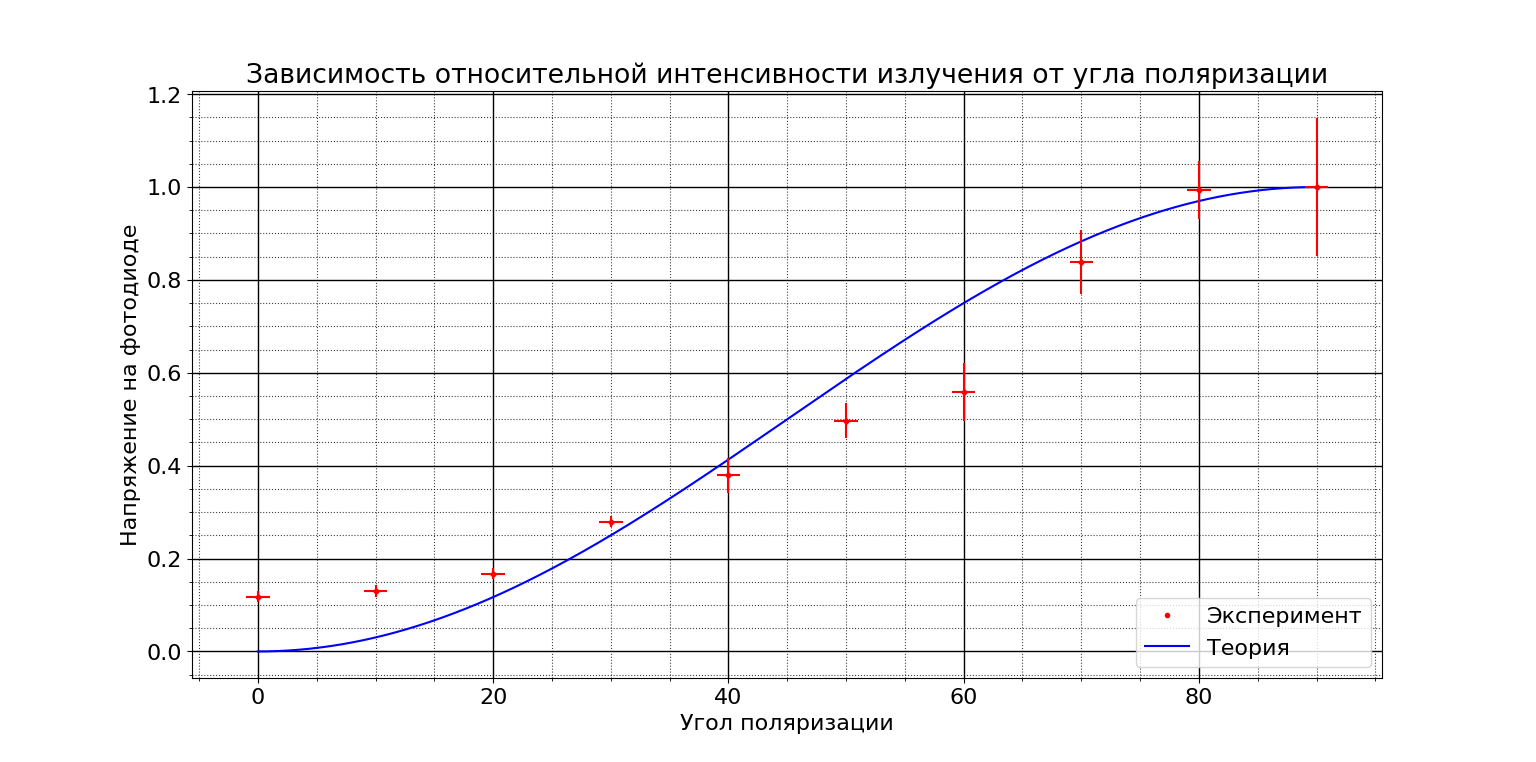
\includegraphics[width=0.9\textwidth]{../Изображения/Поляризация.png}
	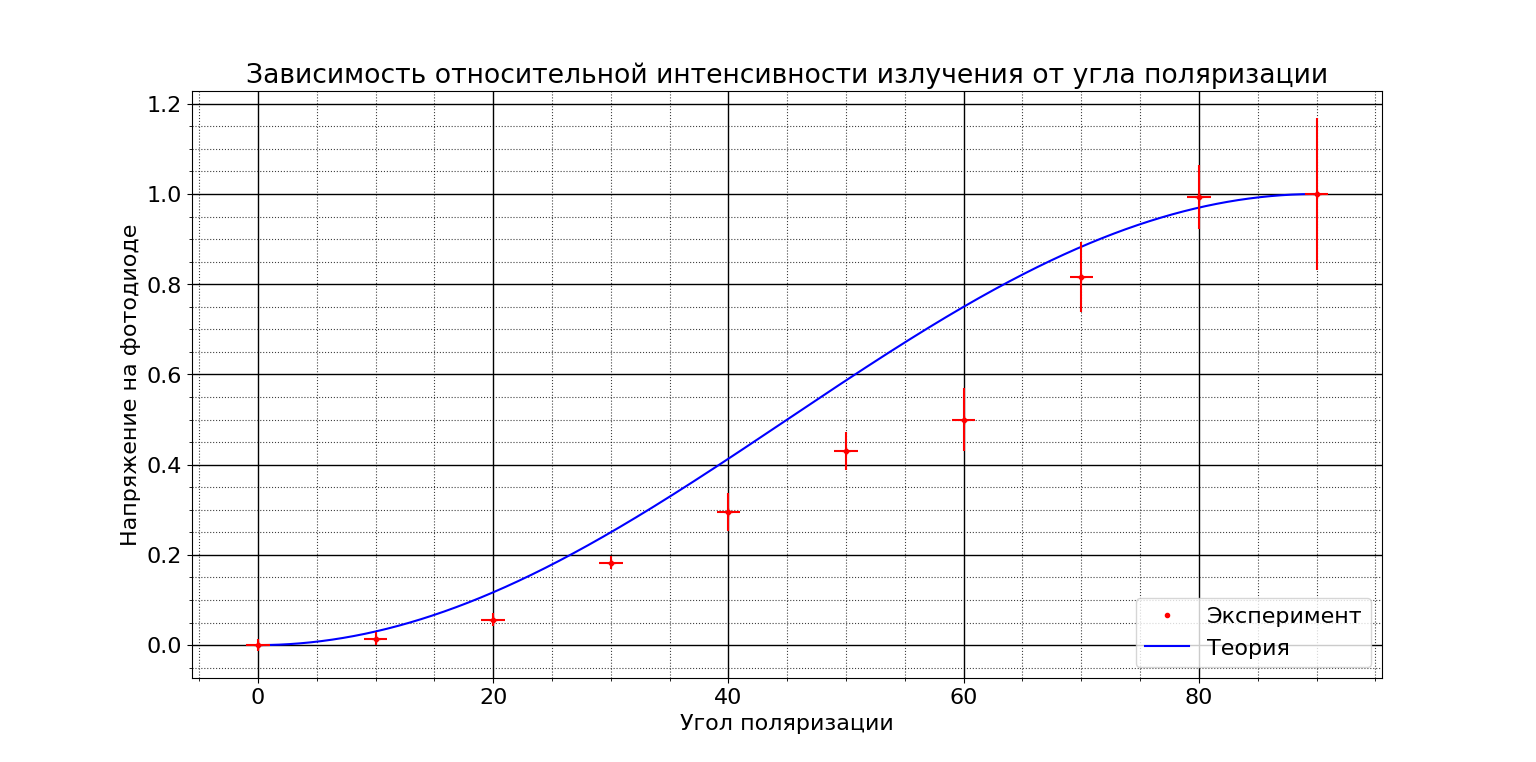
\includegraphics[width=0.9\textwidth]{../Изображения/Поляризация уточненная.png}
\end{figure}


\subsection*{Наблюдение модовой структуры излучения}

\begin{figure}[H]
	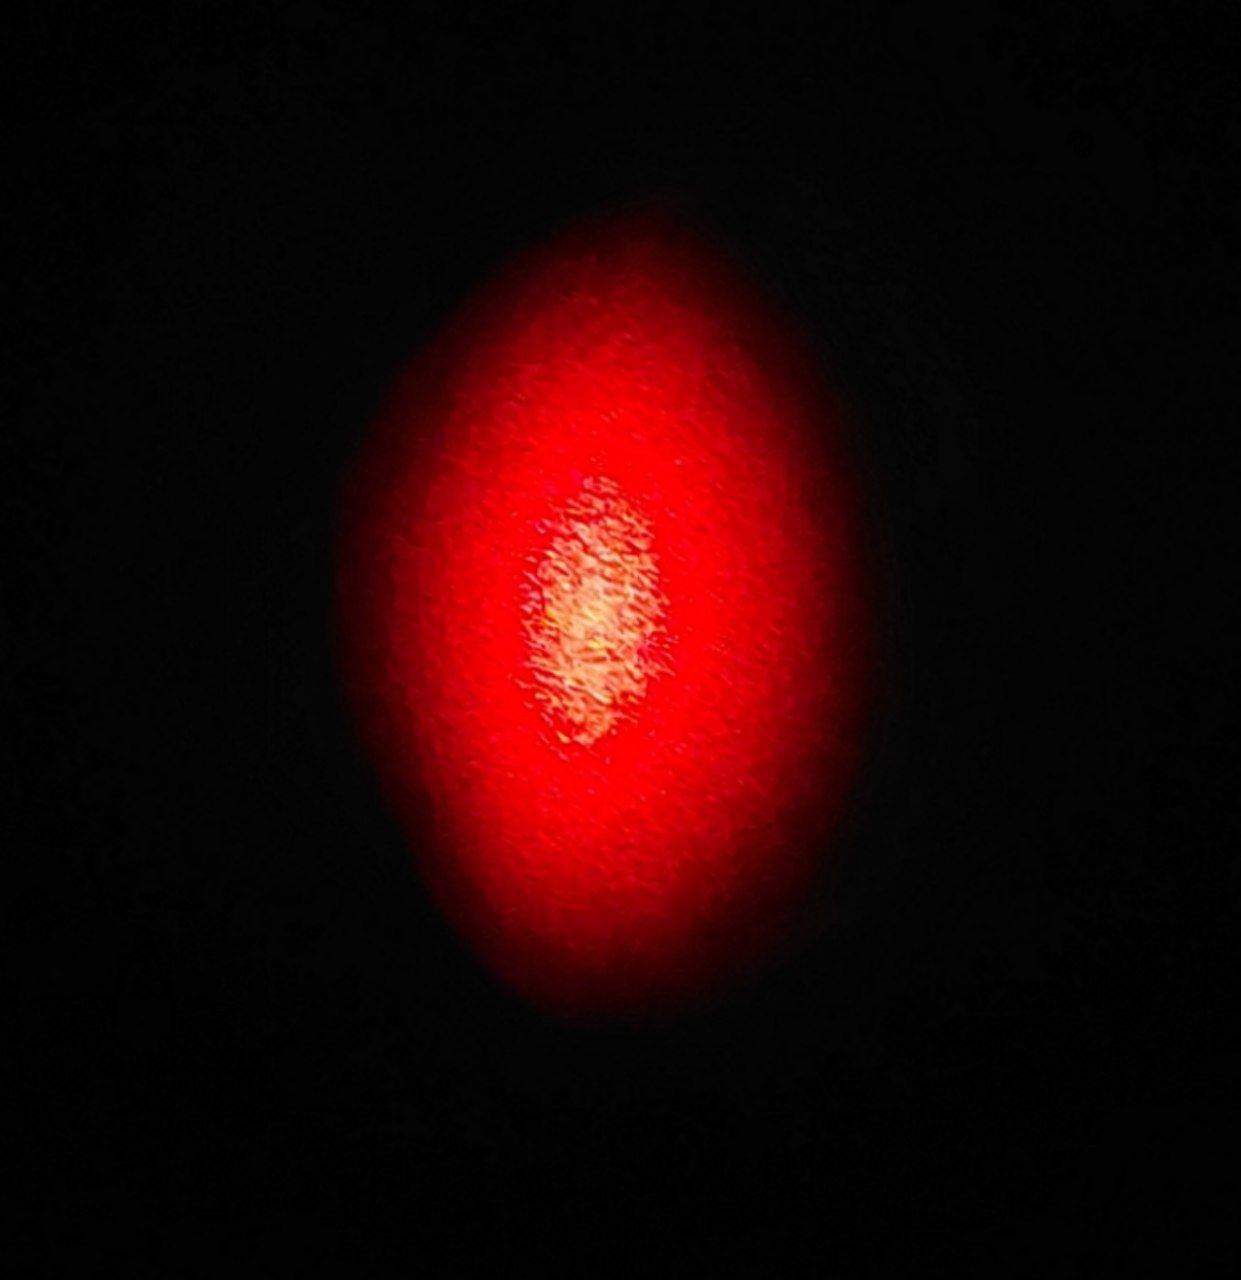
\includegraphics[width=0.33333\textwidth, height = 0.33333\textwidth]{../Изображения/00.jpg}
	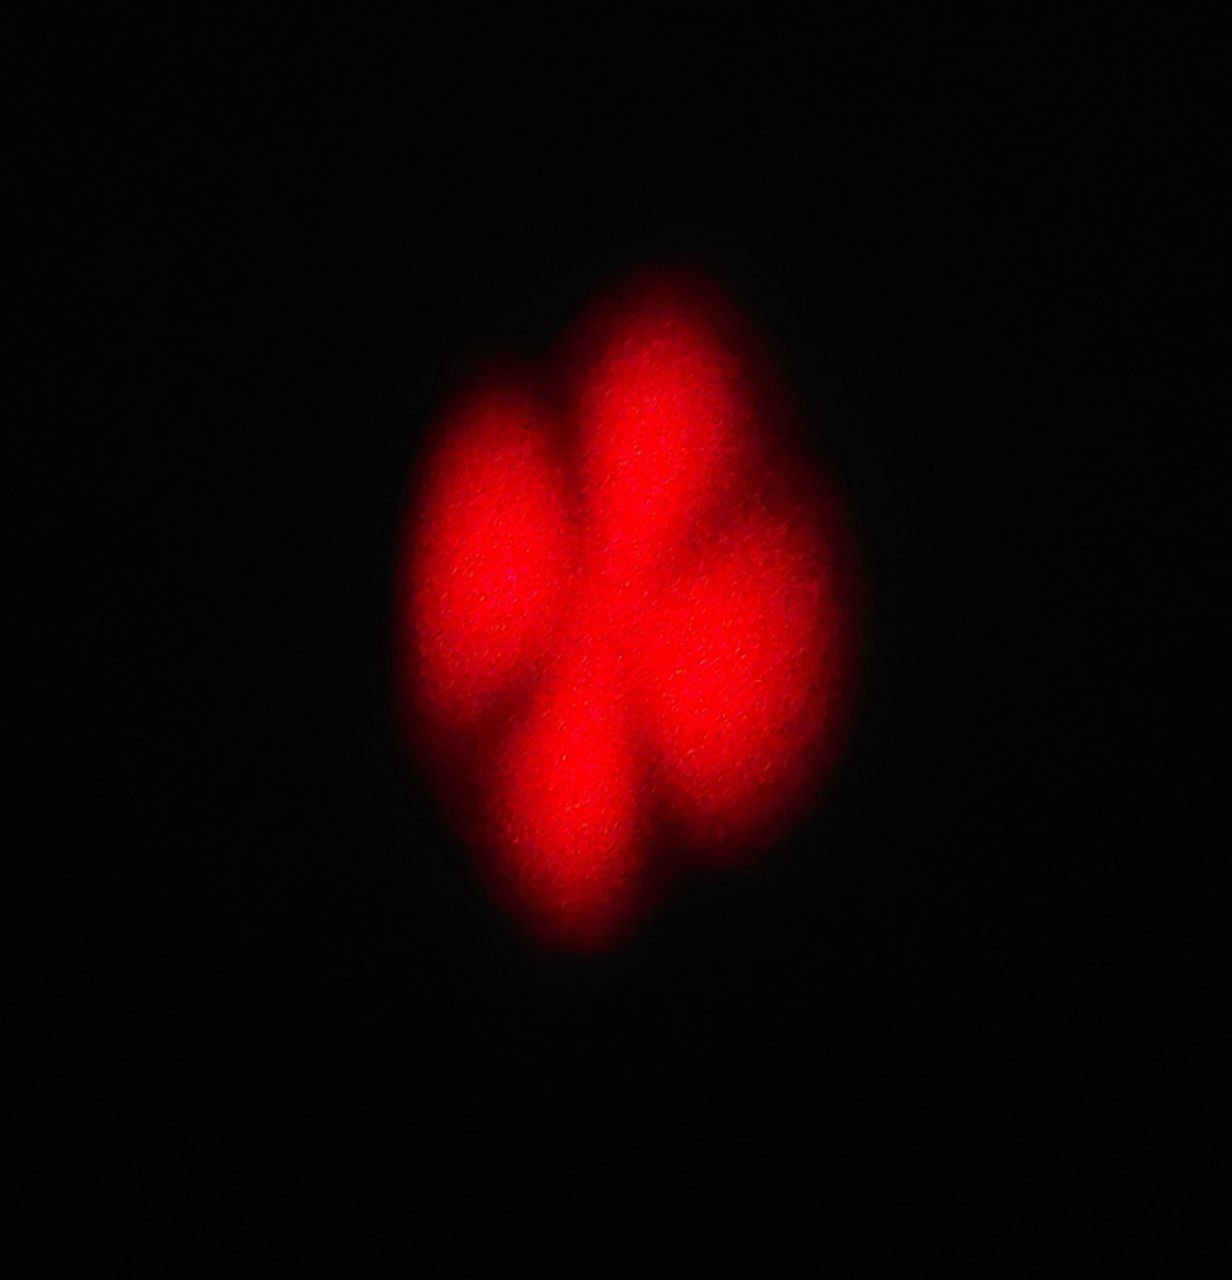
\includegraphics[width=0.33333\textwidth, height = 0.33333\textwidth]{../Изображения/11.jpg}
	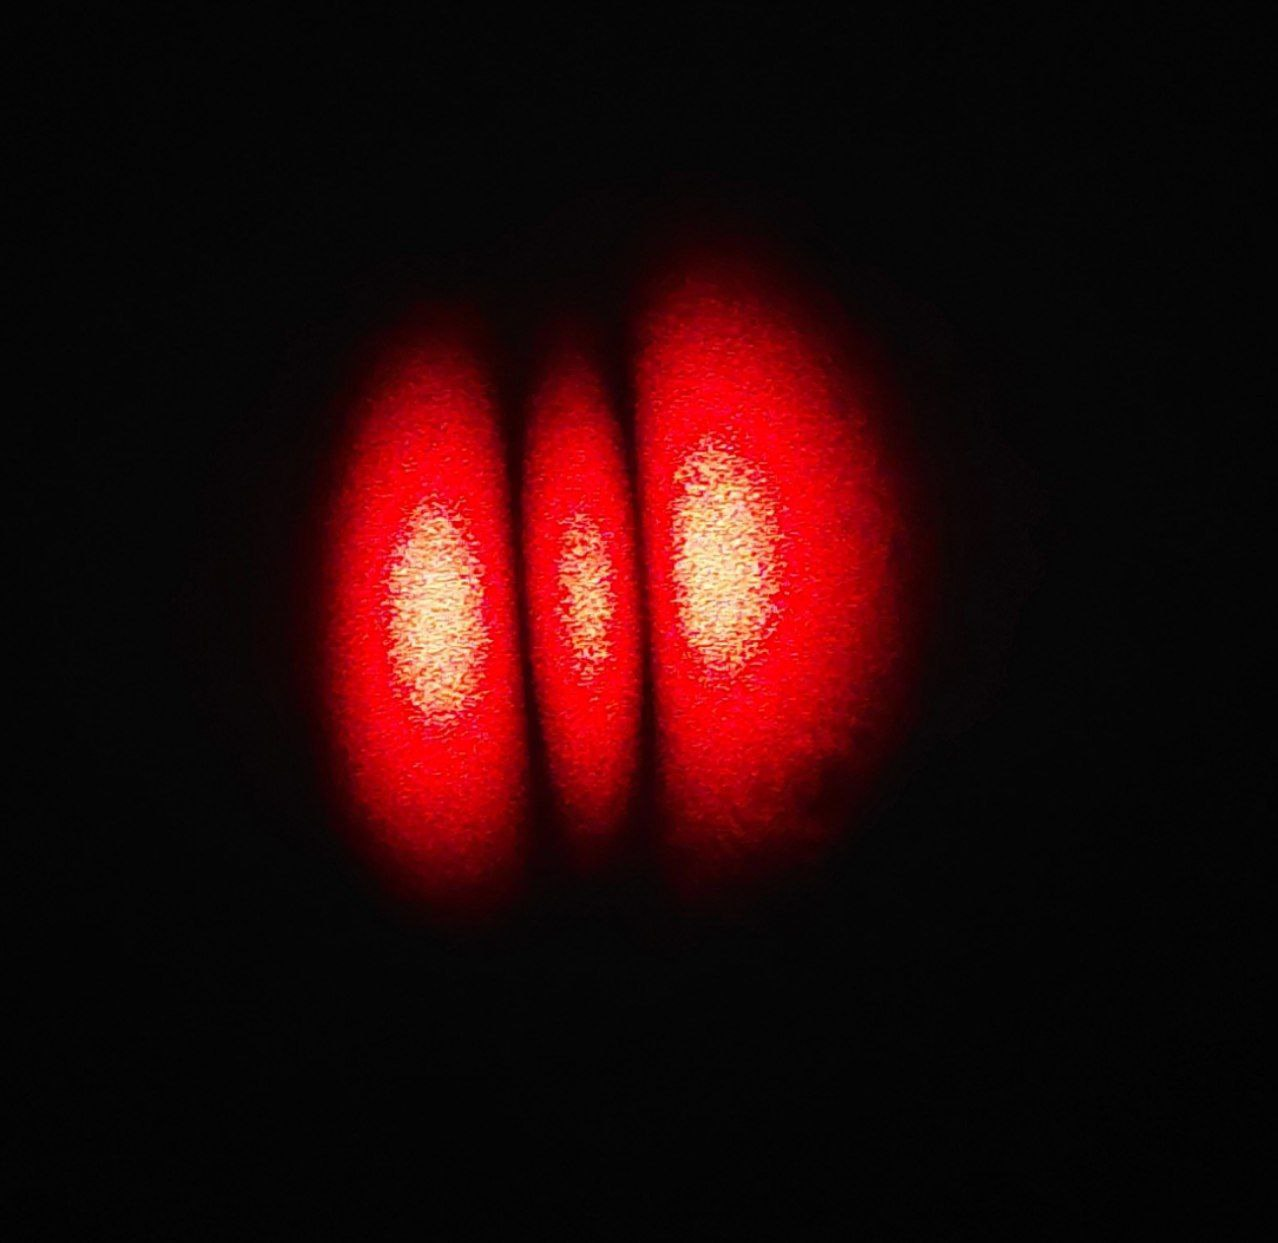
\includegraphics[width=0.33333\textwidth, height = 0.33333\textwidth]{../Изображения/20.jpg}
	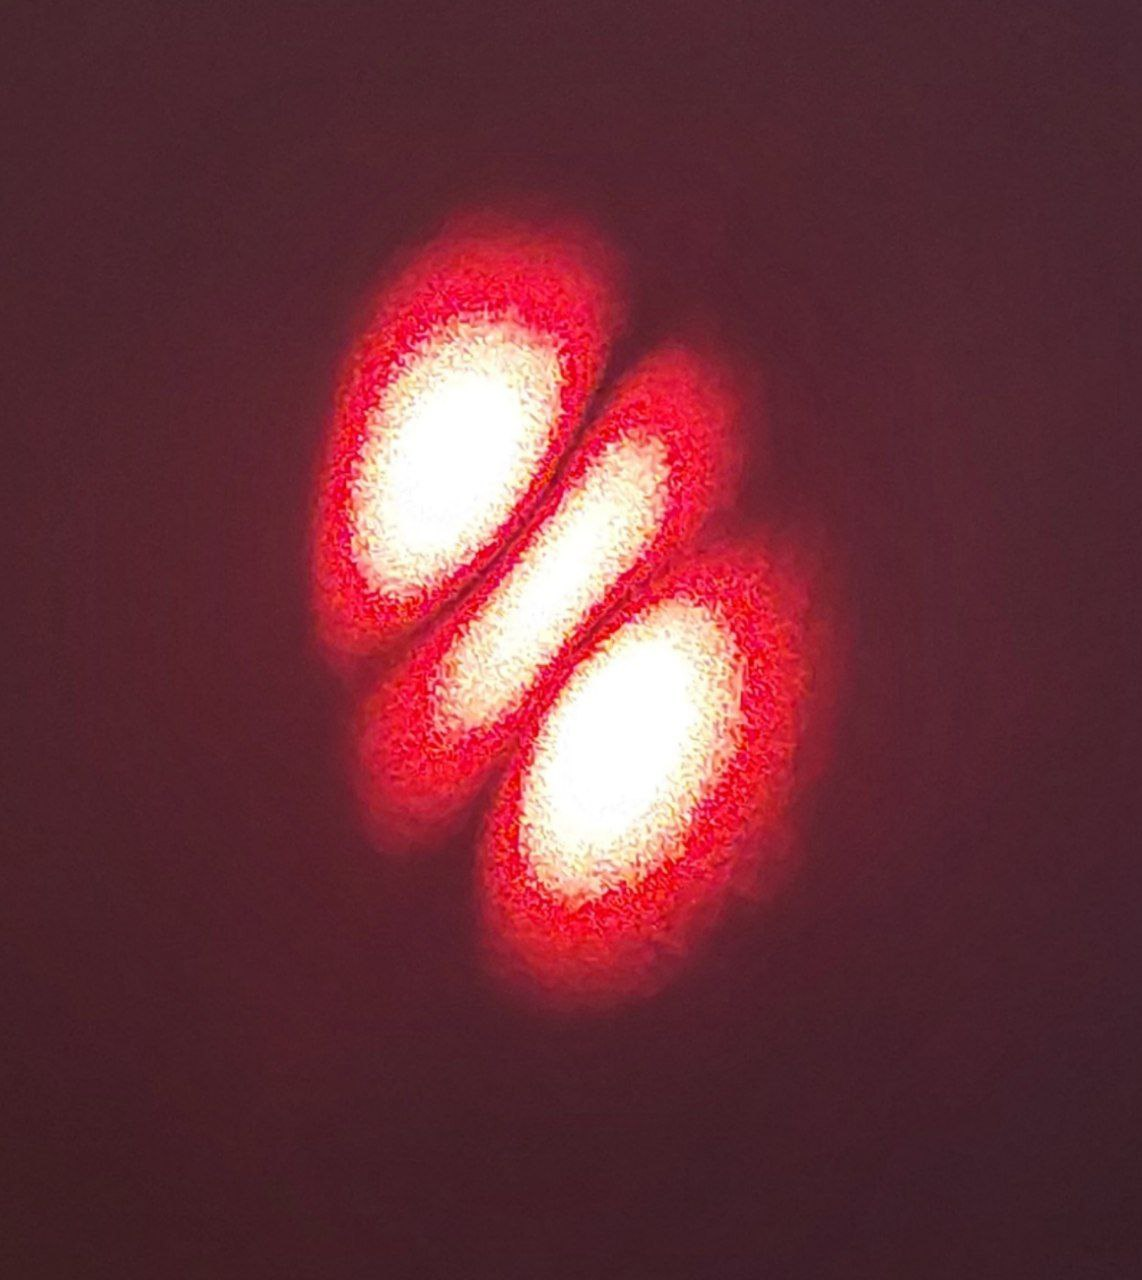
\includegraphics[width=0.33333\textwidth, height = 0.33333\textwidth]{../Изображения/20_2.jpg}
	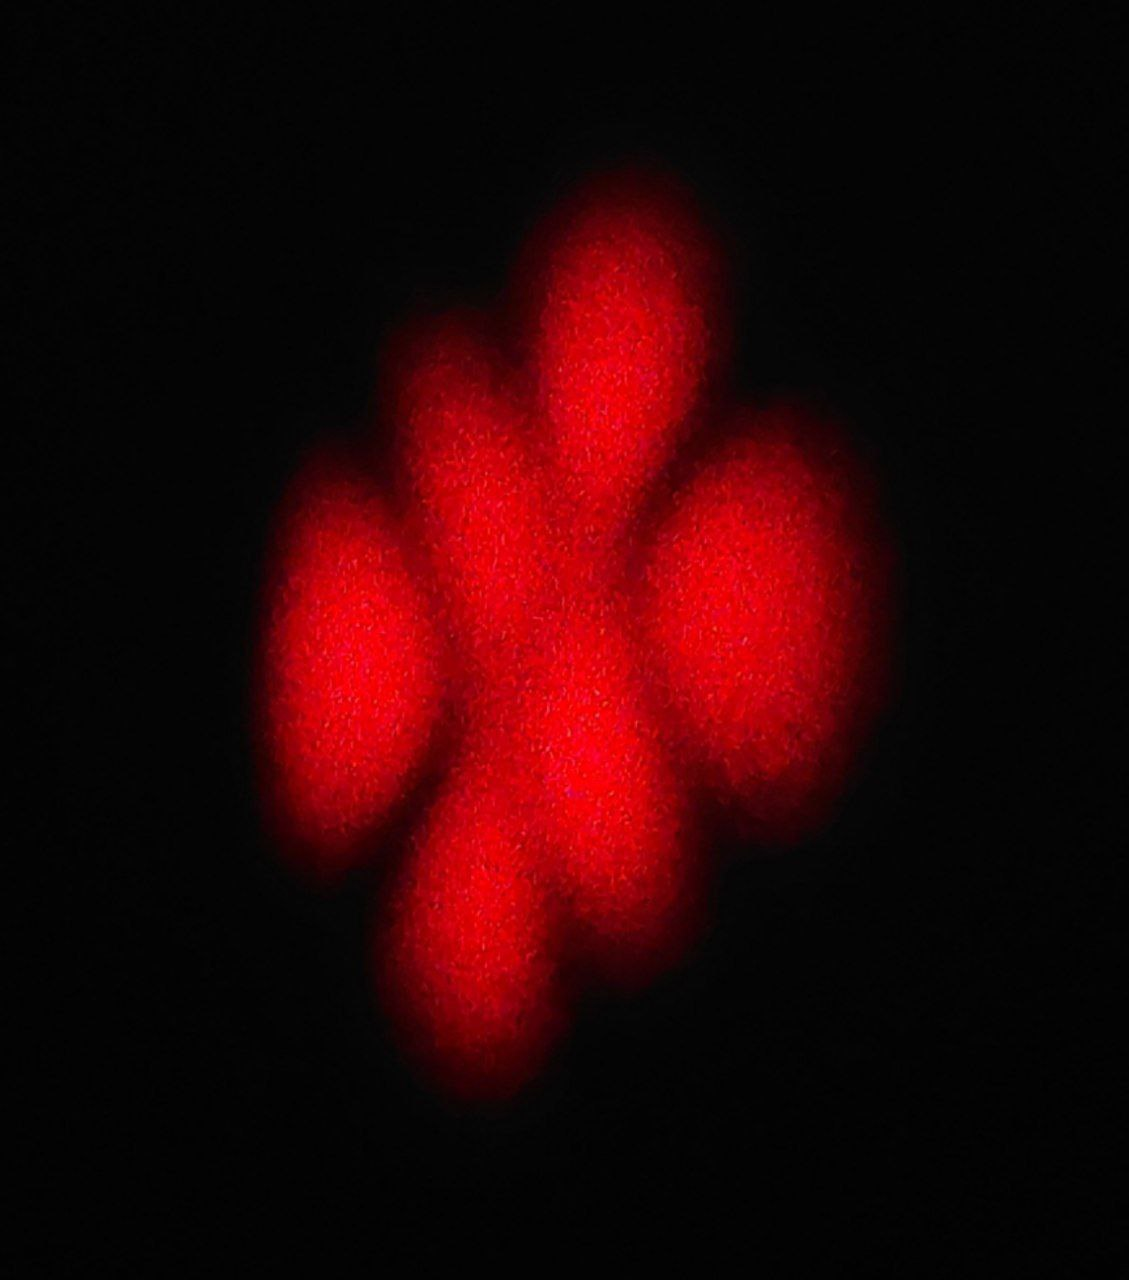
\includegraphics[width=0.33333\textwidth, height = 0.33333\textwidth]{../Изображения/21.jpg}
	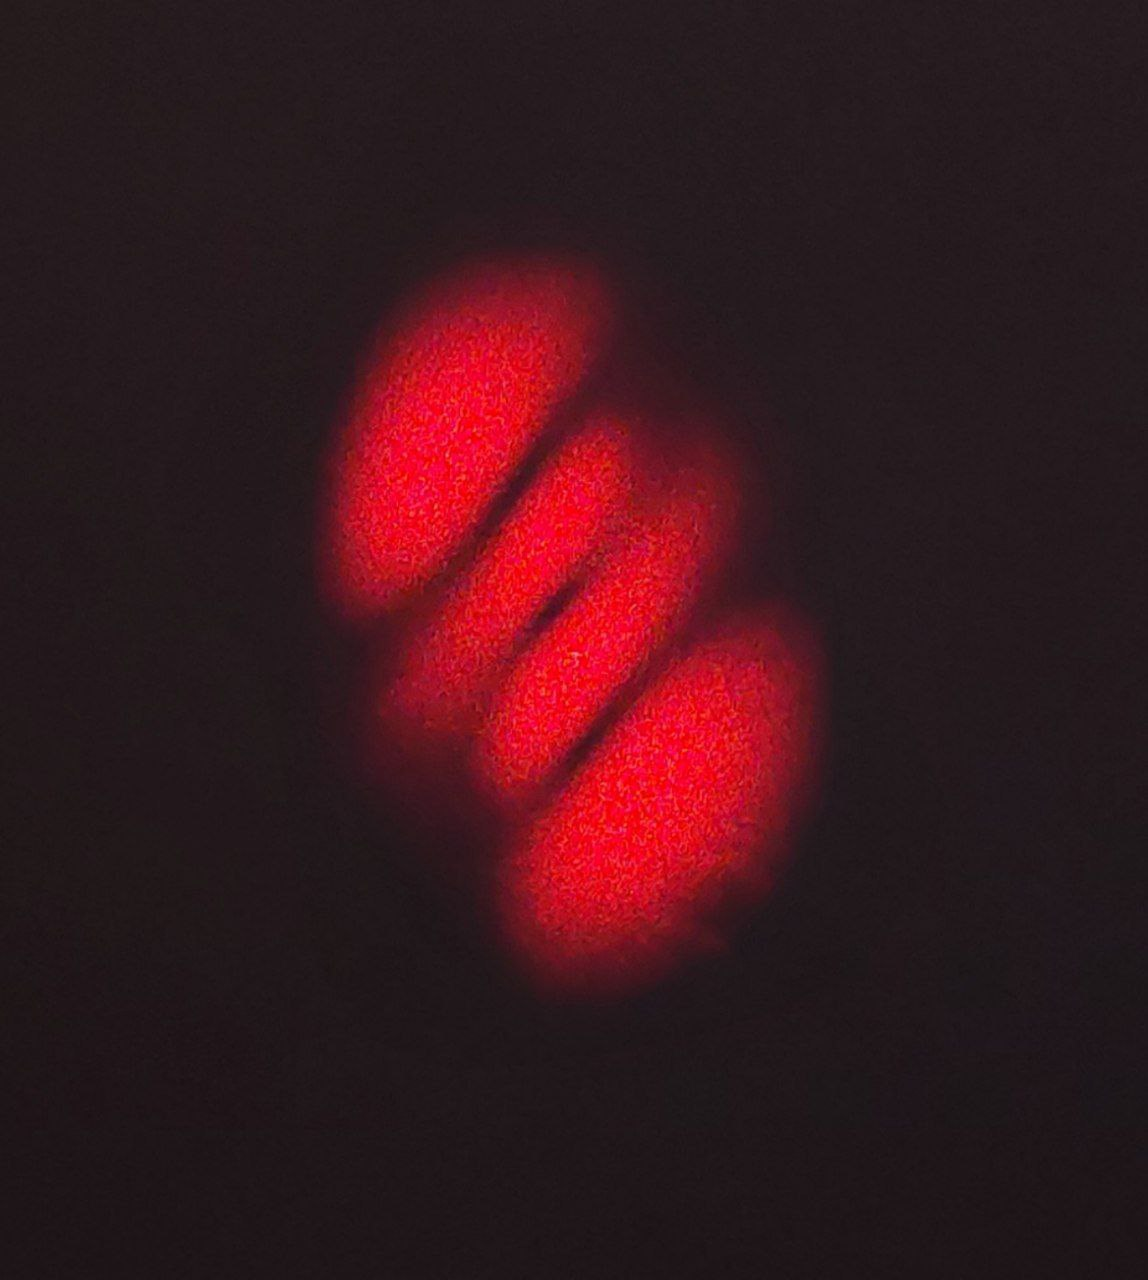
\includegraphics[width=0.33333\textwidth, height = 0.33333\textwidth]{../Изображения/30.jpg}
	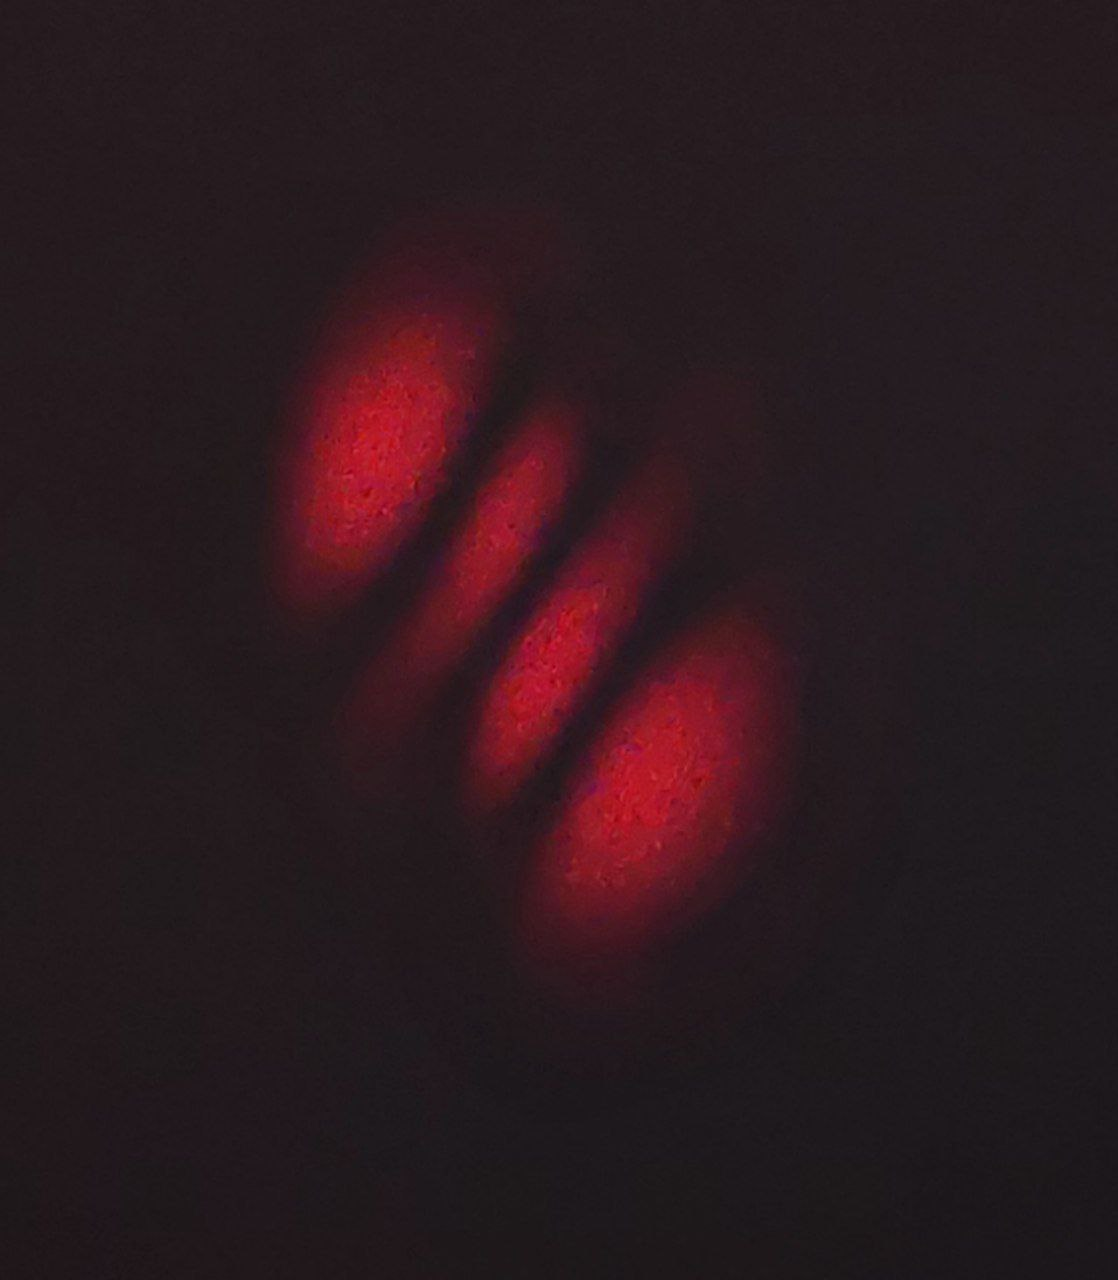
\includegraphics[width=0.33333\textwidth, height = 0.33333\textwidth]{../Изображения/30_2.jpg}
	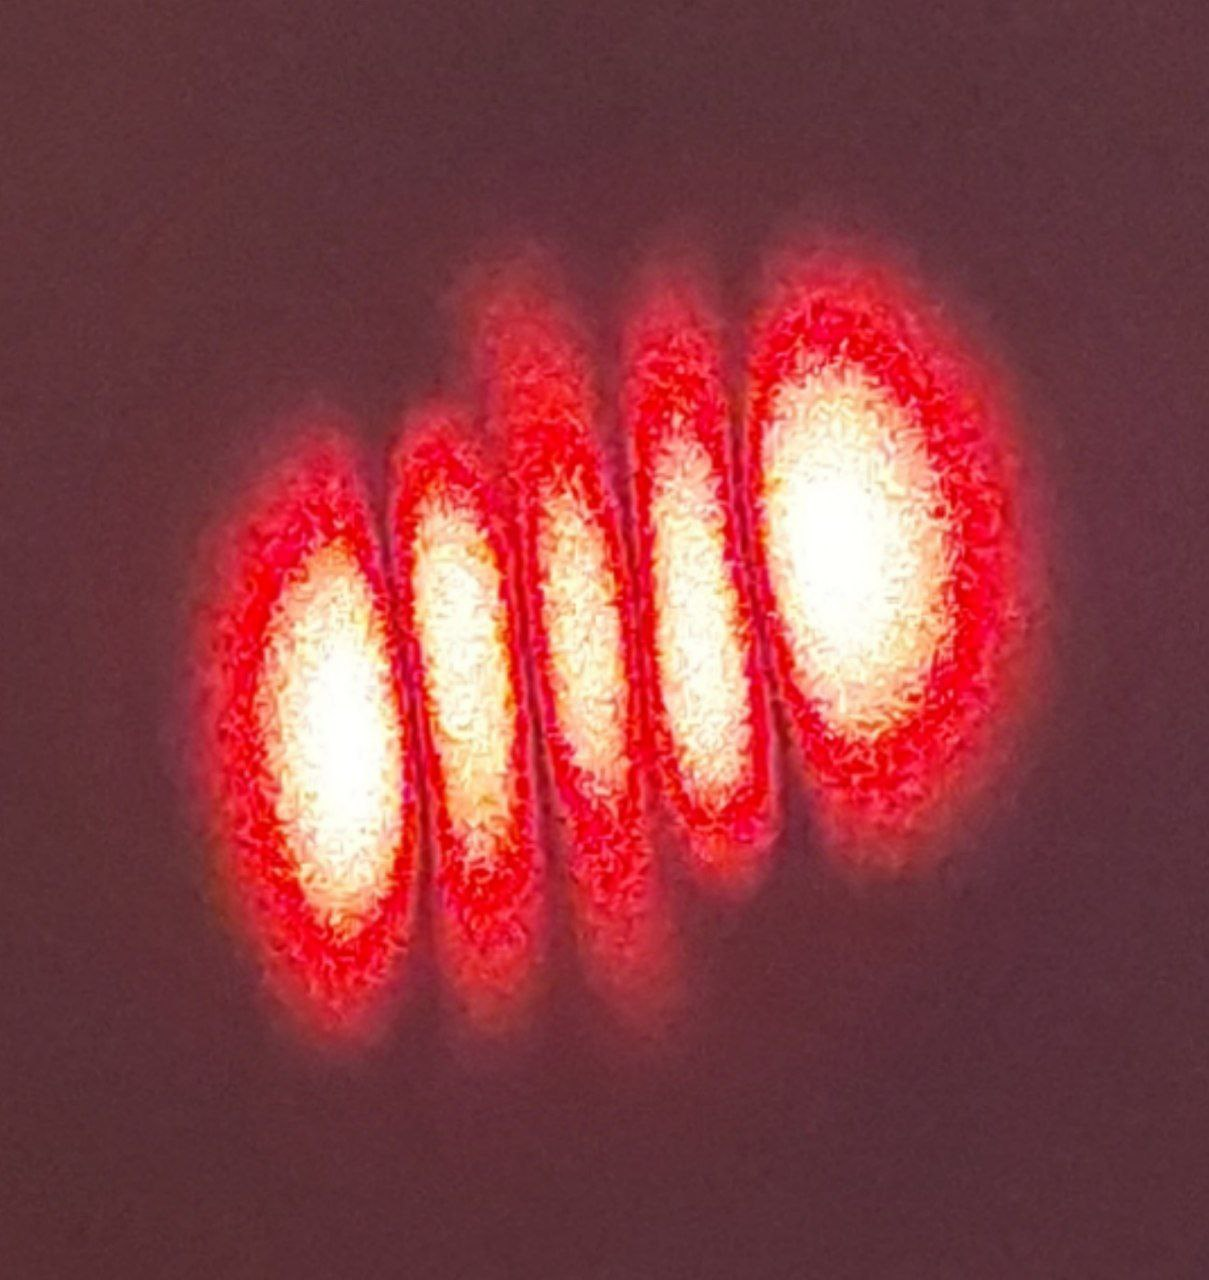
\includegraphics[width=0.33333\textwidth, height = 0.33333\textwidth]{../Изображения/40.jpg}
	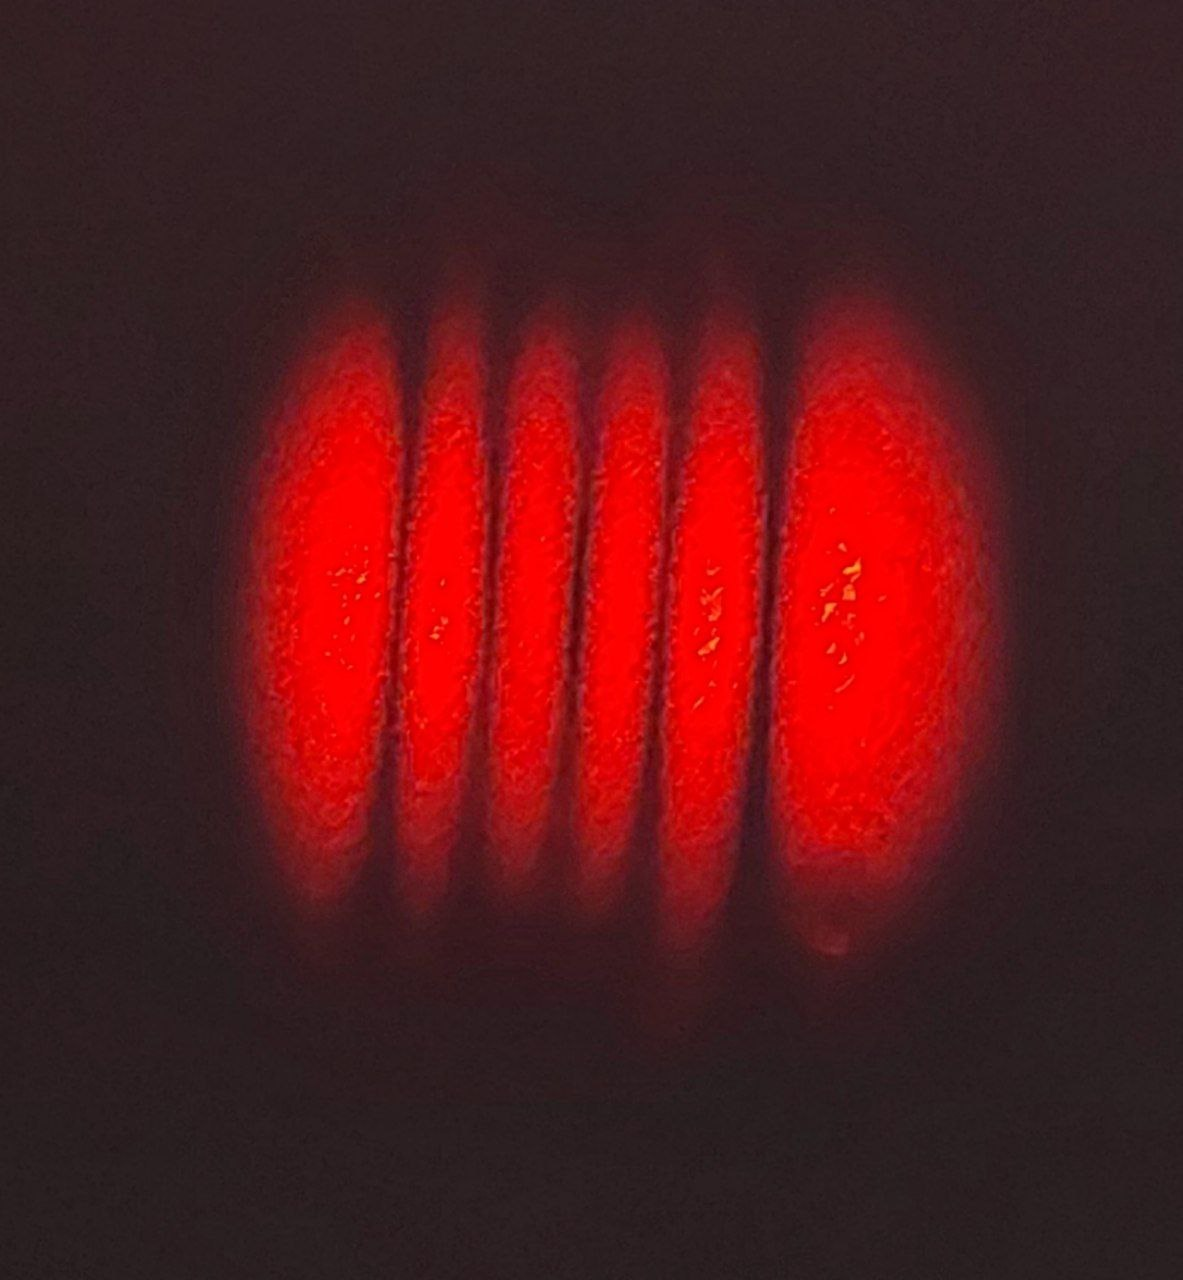
\includegraphics[width=0.33333\textwidth, height = 0.33333\textwidth]{../Изображения/50.jpg}
\end{figure}



